\chapter[Conclusion and Future Work]{Conclusion and Future Work}
\chaptermark{Conclusion}
\label{chap:conclusion}
\minitoc

In this section, we will highlight some of the major contributions that were achieved within this thesis. We will further discuss the major shortcomings as well as future prospectives that could address those limitations. 

On a high level ... we outlined in the introduction


% My thesis showed I did very useful things and also pleases my supervisor~\cite{Ourselin:MICCAI:00}. I also showed that I somewhat address the challenges laid out in \chapref{chap:intro}.


\subsection{Marker-free Unified Eye-hand Calibration}
\label{con:sec:marker_free}

\chapref{chap:registration}

\begin{figure}
    \centering
    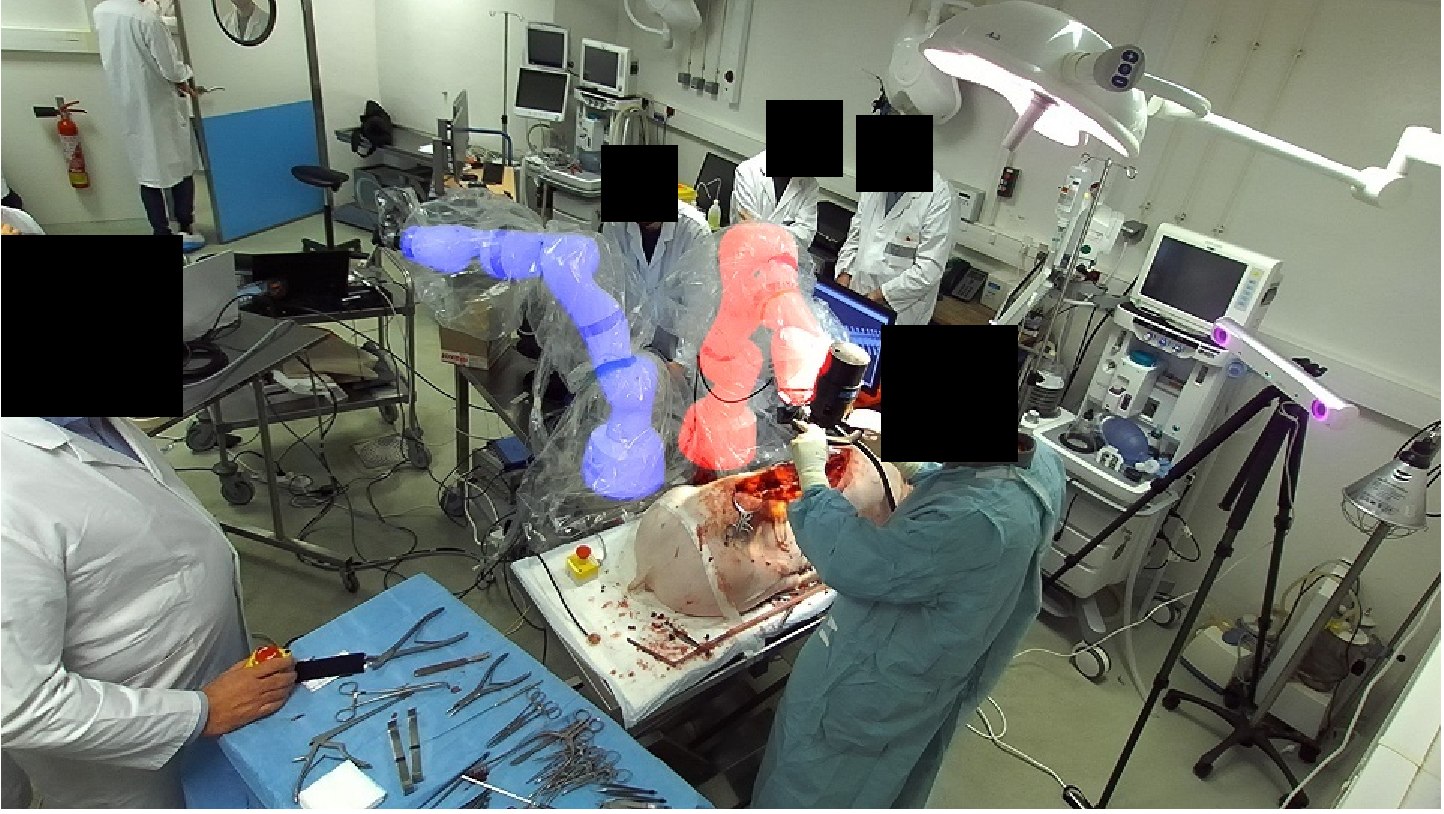
\includegraphics[width=\textwidth]{conclusion/img/draped_ground_truth.pdf}
    \caption{Caption. Refers to \secref{con:sec:marker_free}.}
    \label{con:fig:draped_ground_truth}
\end{figure}

- differentiable rendering -> solving draped robots

\subsection{Visual Servo}
\label{con:sec:visual_servo}
\chapref{chap:robotic_endoscope}
- QP or other solvers

\subsection{Homography Estimation}
\label{con:sec:hom_est}

\chapref{chap:camera_motion_extraction}
- novel view synthesis
    - runtime for data
    - no diffusion models \cite{rombach2022high} as these tend to hallucinate and iterative  
\begin{figure}
    \centering
    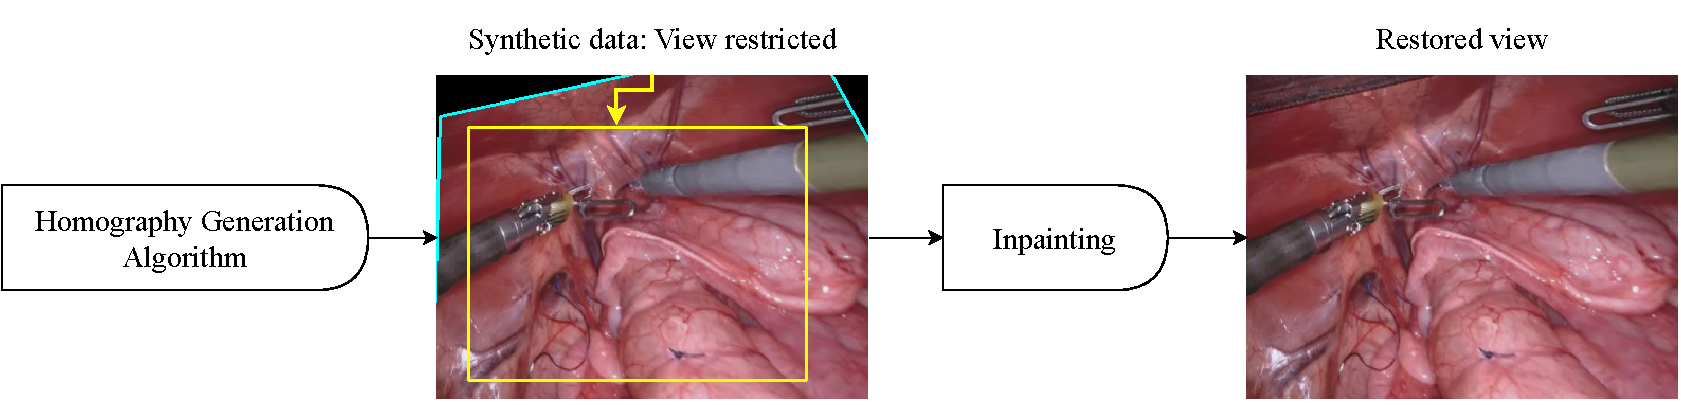
\includegraphics[width=\textwidth]{conclusion/fig/fourier_inpainting.pdf}
    \caption{Algorithm from \secref{c3:sec:hom_gen} \figref{c3:fig:hom} Caption \cite{suvorov2021resolution}. Refers to \secref{con:sec:hom_est}.}
    \label{con:fig:inpainting}
\end{figure}
- incorporate depth \cite{budd2024transferring}: novel view synthesis
- utilize inpainting methods as well
- inpainting -> better range


\subsection{Homography Prediction}
\label{con:sec:hom_pred}

\chapref{chap:camera_motion_prediction}

- rl on-top (force controlled rcm, rlhf)
- bootstrapping motion:
    - visual qa
- llm interface models: \figref{in:fig:hypothesized_pipeline} (beyond scope)
